\documentclass[a4paper,12pt]{article}

% Margins
\usepackage{geometry}
\geometry{left=25mm,right=25mm,%
bindingoffset=0mm, top=20mm,bottom=20mm}

% More Math Symbols
\usepackage{amssymb}

% Trademark Symbols
\usepackage{textcomp}

% Text in math
\usepackage{amsmath}

% For Diagrams
\usepackage{graphicx}
\usepackage{wrapfig}

% Footnote URLs
\usepackage{hyperref}

% Underlines
\usepackage{soul}

% Font
\usepackage{anyfontsize}
%\usepackage[default,regular,black]{sourceserifpro}
\usepackage{tgpagella,eulervm}
\usepackage[T1]{fontenc}

% Mutli-column text
\usepackage{multicol}

% For tables
\usepackage[table]{xcolor}
\usepackage{array}
\usepackage{tablefootnote}

% code listing settings
\usepackage{listings}
\usepackage[space=true]{accsupp}
\newcommand{\noncopynumber}[1]{
    \BeginAccSupp{method=escape,ActualText={}}
    #1
    \EndAccSupp{}
}
\definecolor{codegreen}{rgb}{0,0.6,0}
\definecolor{codegray}{rgb}{0.5,0.5,0.5}
\definecolor{inlinecode}{rgb}{0.1,0.1,0.1}
\definecolor{codepurple}{rgb}{0.58,0,0.82}
\definecolor{backcolour}{rgb}{0.95,0.95,0.92}
\lstset{
    language=Python,
    basicstyle=\ttfamily\small,
    aboveskip={1.0\baselineskip},
    breakatwhitespace=false,         
    keepspaces=true,
    belowskip={1.0\baselineskip},
    columns=fullflexible,
    extendedchars=true,
    breaklines=true,
    tabsize=4,
    frame=lines,
    showtabs=false,
    showspaces=false,
    showstringspaces=false,
    commentstyle=\color{codegray},
    keywordstyle=\bfseries,
    %stringstyle=\rmfamily,
    numbers=none,
    numberstyle=\color{codegray}\footnotesize\noncopynumber,
    stepnumber=1,
    numbersep=10pt,
    captionpos=t,
    escapeinside={\%*}{*)},
}


\lstdefinestyle{output}{
    basicstyle=\ttfamily\small,
    aboveskip={1.0\baselineskip},
    breakatwhitespace=false,         
    keepspaces=true,
    belowskip={1.0\baselineskip},
    columns=fullflexible,
    extendedchars=true,
    breaklines=true,
    tabsize=4,
    frame=lines,
    showtabs=false,
    showspaces=false,
    showstringspaces=false,
    captionpos=t
}
%%%----------%%%----------%%%----------%%%----------%%%

% Title
\newcommand{\linia}{\rule{\linewidth}{0.5pt}}
\makeatletter
\renewcommand{\maketitle}{
\begin{center}
\vspace{2ex}
{\huge \textbf{\@title}}
\vspace{1ex}
\\
\linia\\
\textsf{\@date \hfill
\@author}
\vspace{4ex}
\end{center}
}
\makeatother
% Multicol TOC
\linespread{1.2}
\makeatletter
\renewcommand\tableofcontents{%
    \section*{\makebox[\linewidth][c]{\contentsname}%
      \@mkboth{\MakeUppercase\contentsname}{\MakeUppercase\contentsname}}%
    \begin{multicols}{2}%
    \@starttoc{toc}%
    \end{multicols}
    }
\makeatother

% Short negative symbol in math mode (sub-zero mnemonic)
\newcommand{\sz}{\text{-}}


% Names
\newcommand{\esp}{\texttt{ESP-32WROOM}}
\newcommand{\con}{\textit{Console}}

% Headers
\usepackage{fancyhdr}
\usepackage{lastpage}
\pagestyle{fancy}
\lhead{}
\chead{}
\rhead{}
\lfoot{Final Project}
\cfoot{}
\rfoot{Page \thepage \ of \pageref{LastPage}}
\renewcommand{\headrulewidth}{0pt}
\renewcommand{\footrulewidth}{0pt}

\begin{document}
% Setting the fontsize
\fontsize{14}{16}\selectfont

\title{Final Project --- AU Robotics}

\date{29/10/2024}

\author{\textbf{Team B}}

\maketitle

\section*{Preface}

This report serves as a technical overview of everything that has been worked on in the past two weeks by Team B in the final project for AU Robotics in 2024.\\

\fontsize{10}{13}\selectfont
\tableofcontents
\fontsize{14}{16}\selectfont
\newpage
\part{Software}
\section{Overview \& Dataflow} \label{dataflow}
\subsection{Motion Dataflow} \label{motflow}
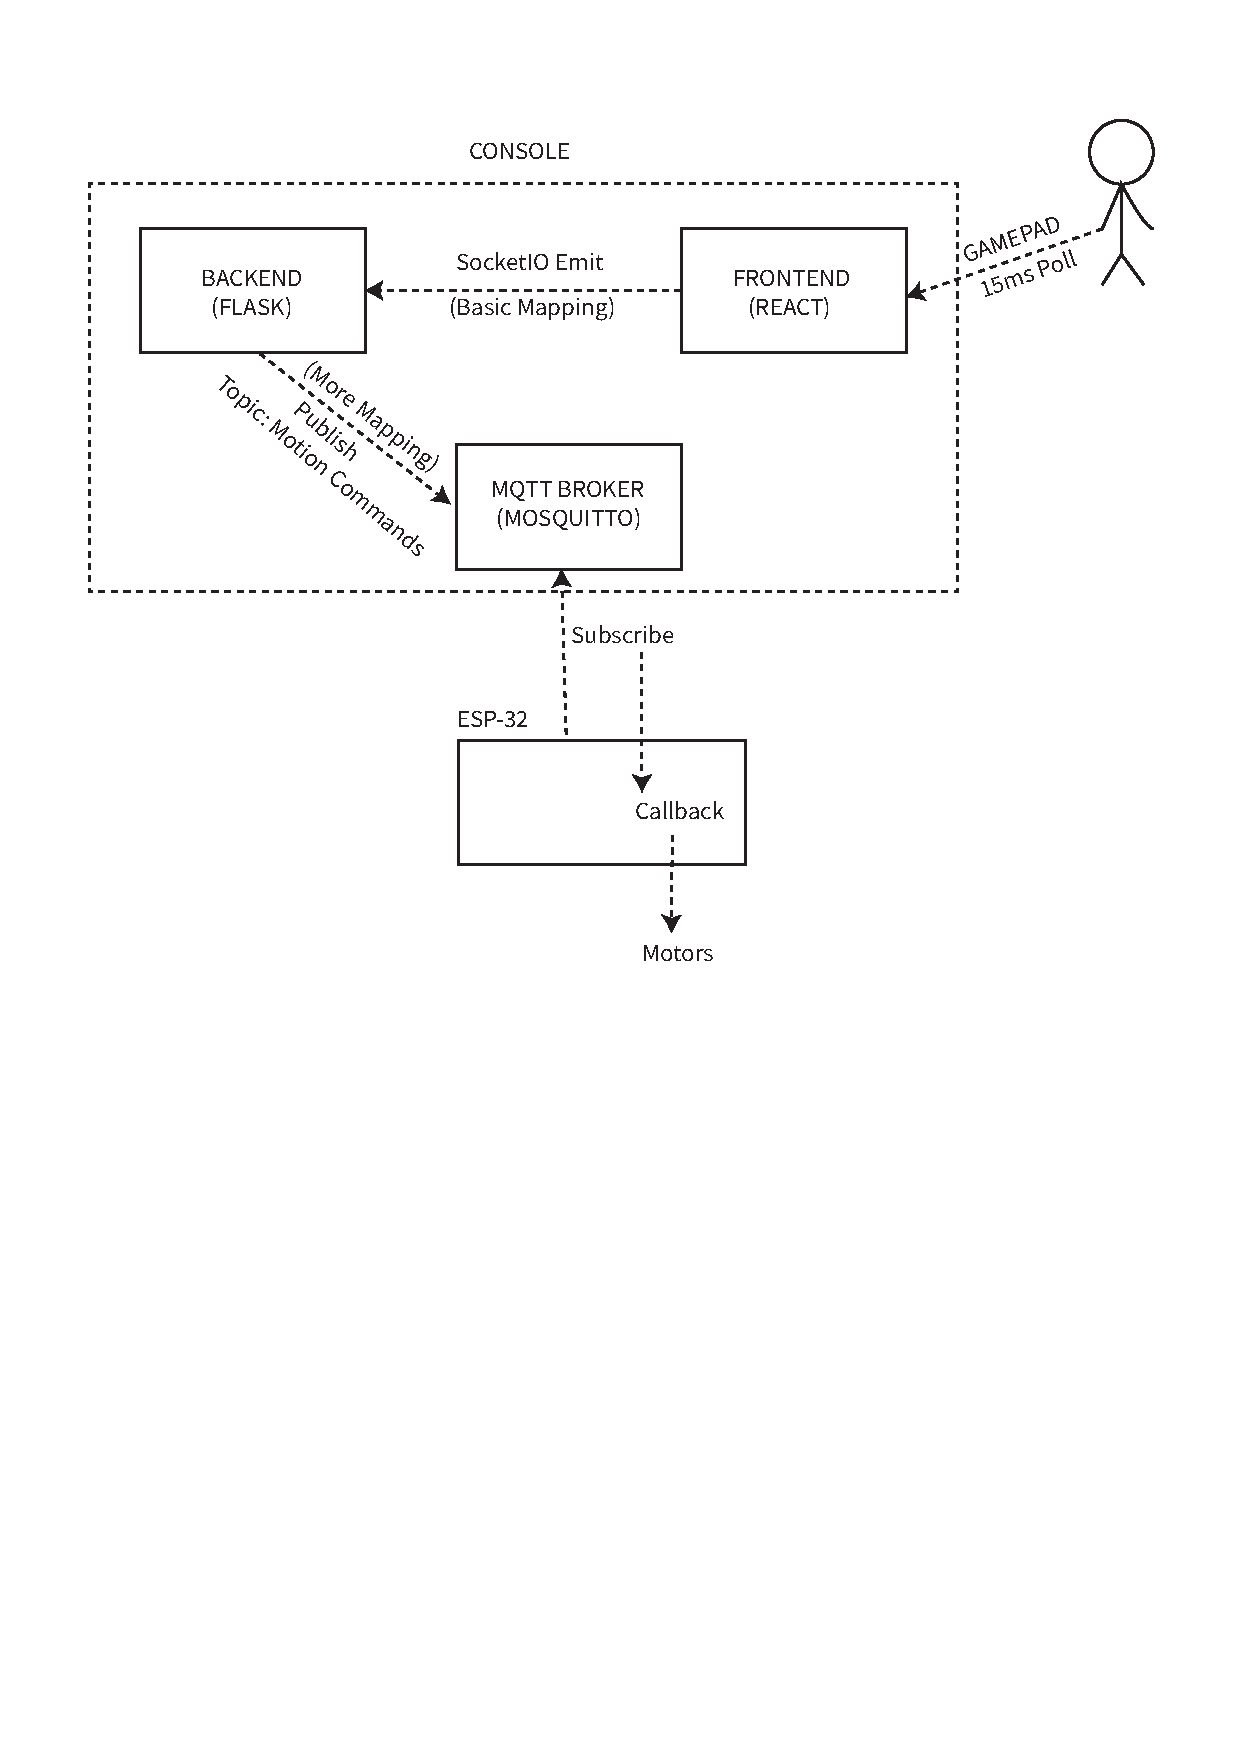
\includegraphics[trim=40 380 0 57,scale=0.95,clip]{media/mot.pdf}

\subsection{Localization Dataflow} \label{locflow}
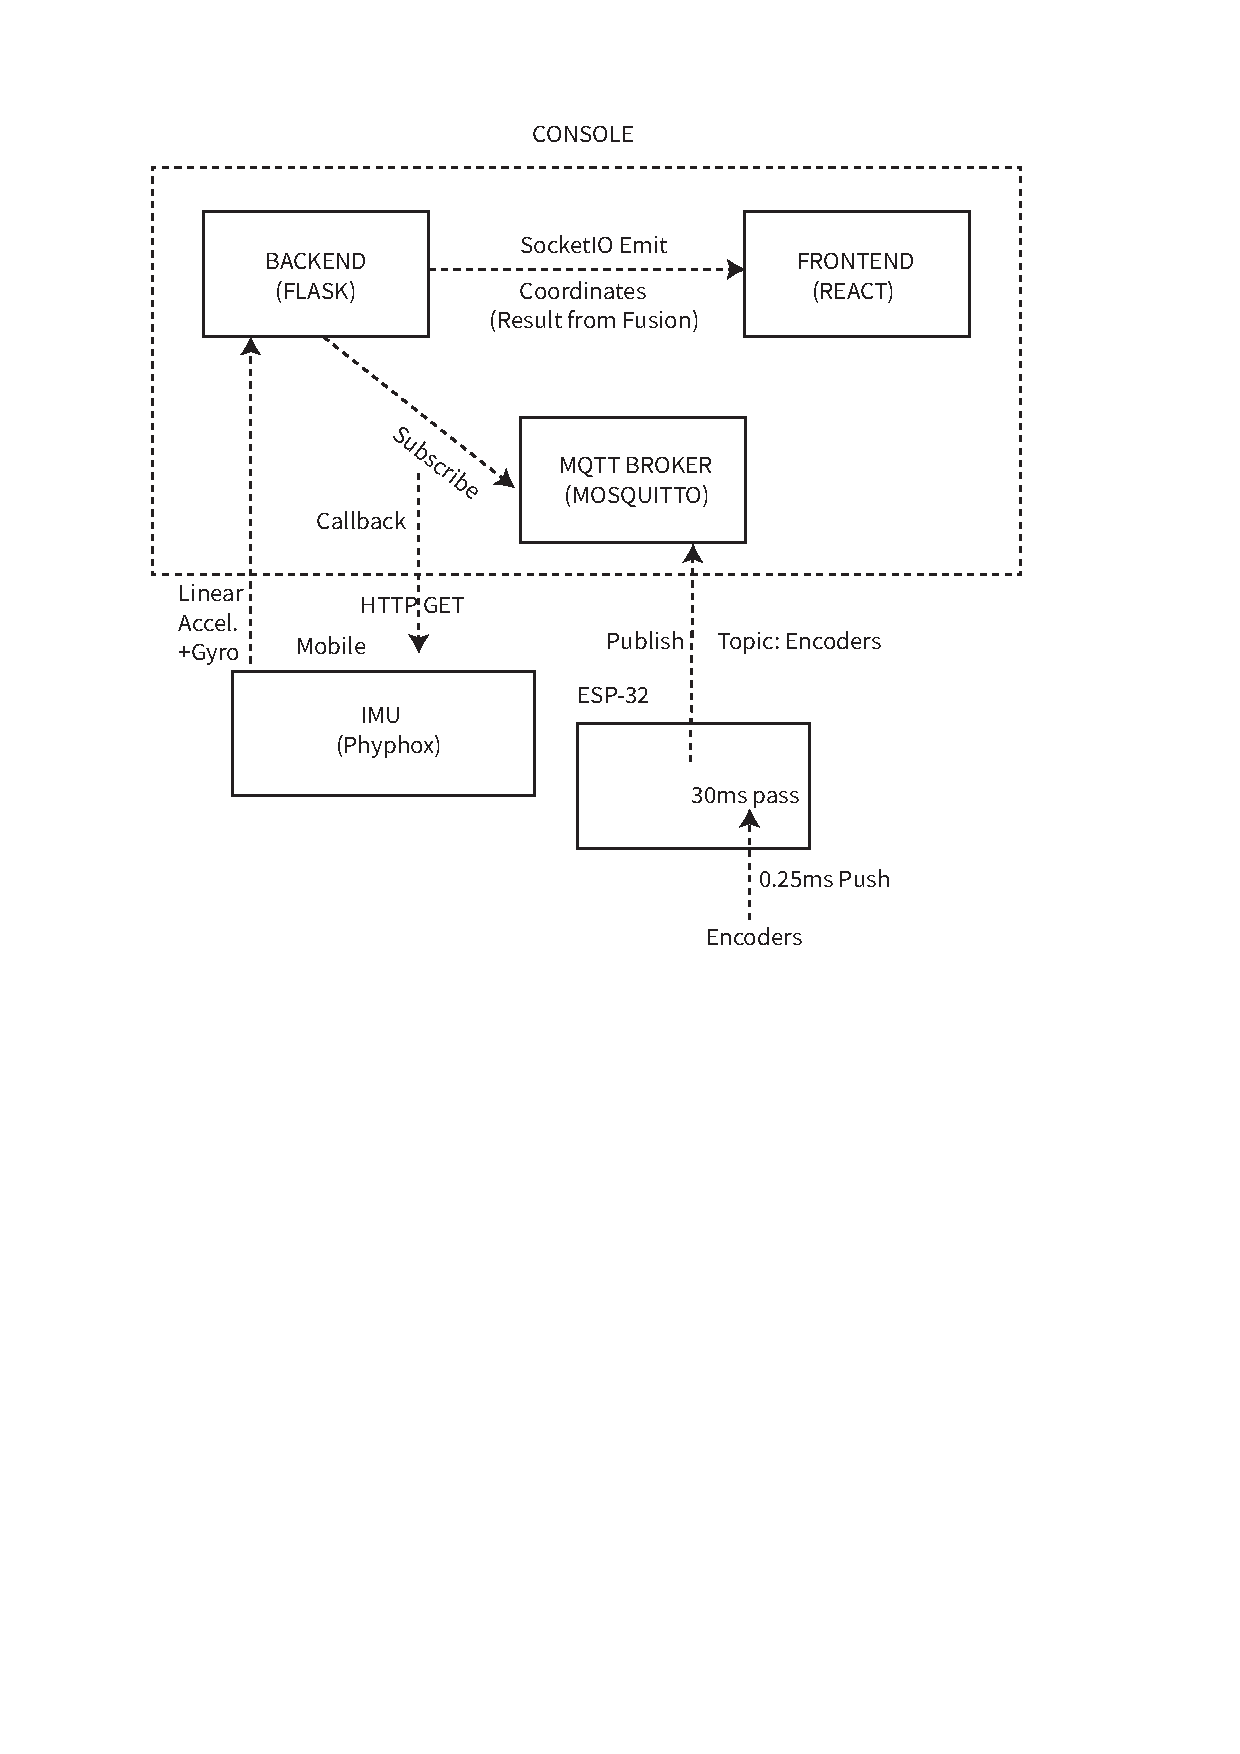
\includegraphics[trim=40 380 0 57,scale=0.95,clip]{media/loc.pdf}

\subsection{Computer Vision Dataflow} \label{visflow}
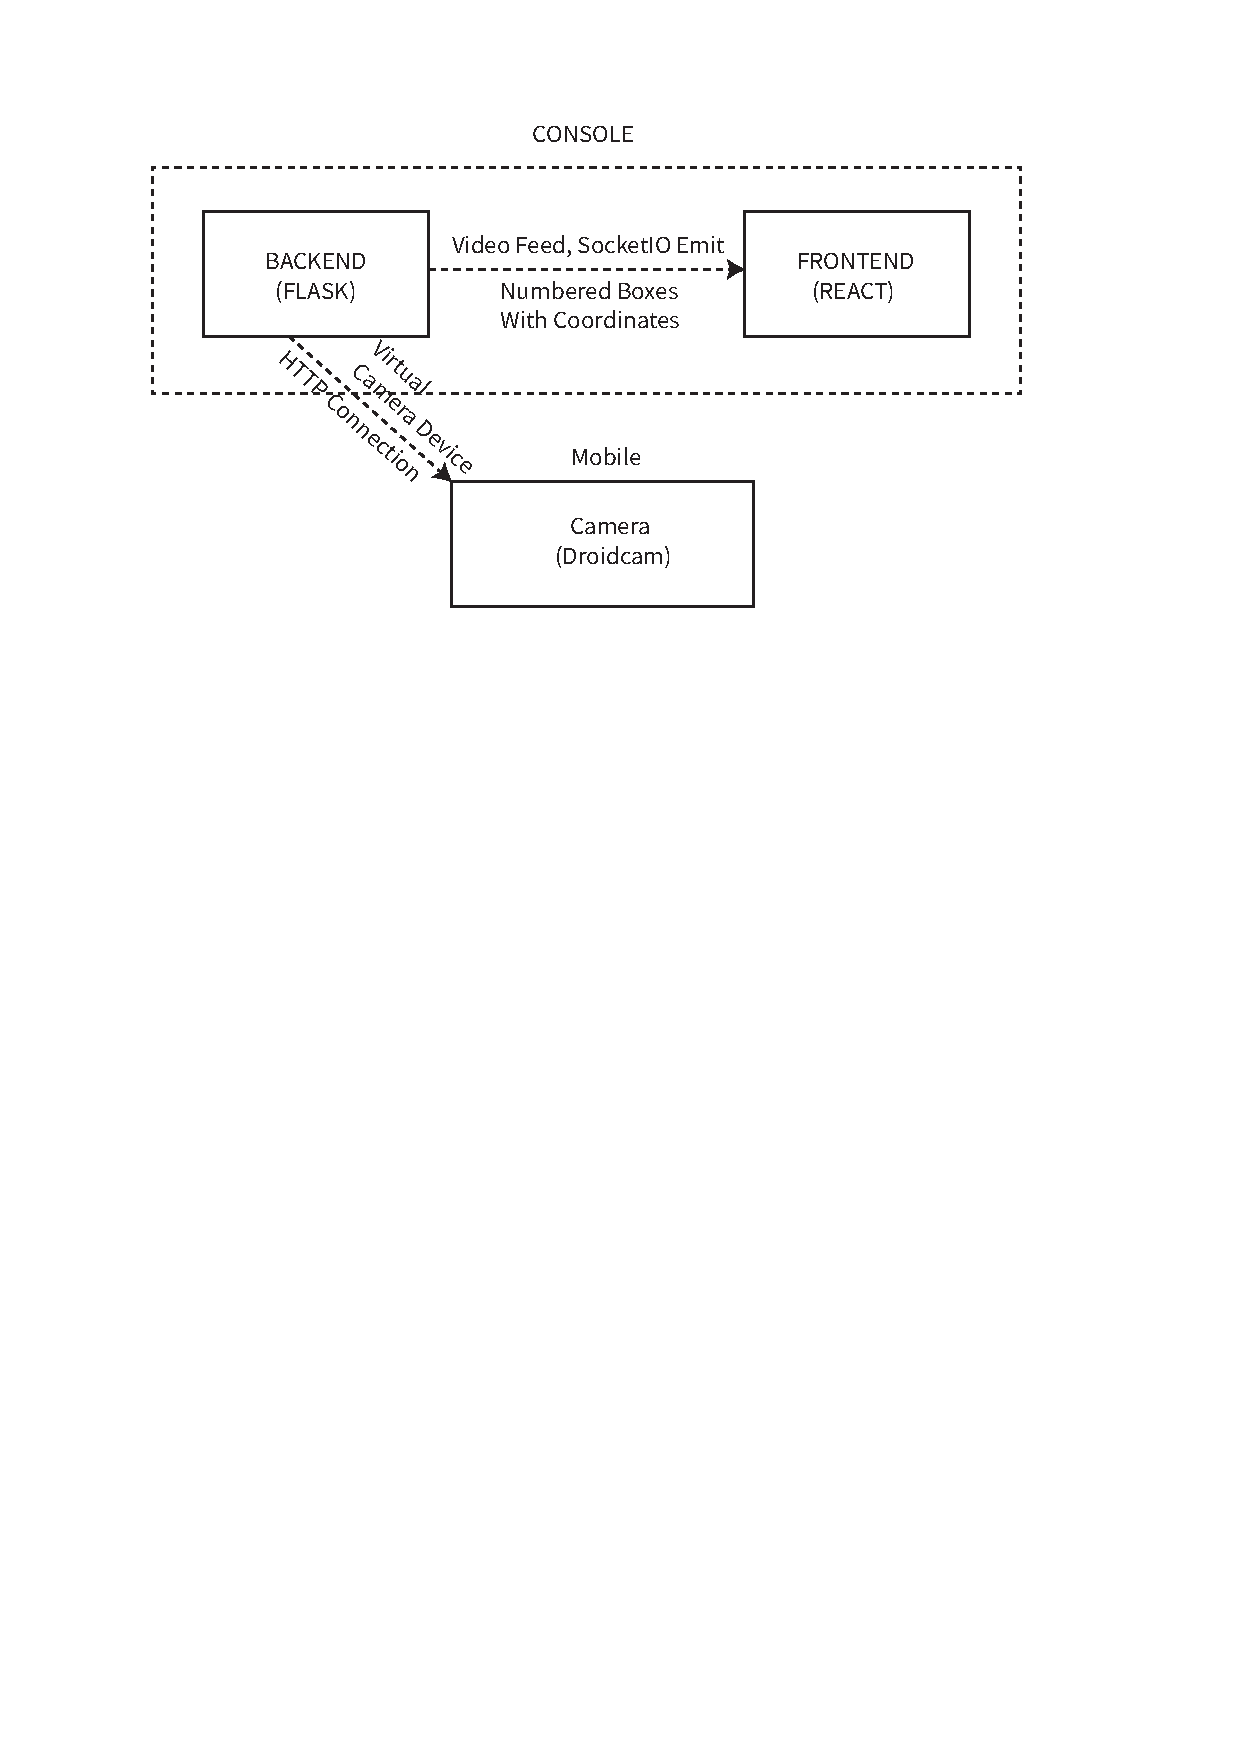
\includegraphics[trim=40 550 0 57,scale=0.95,clip]{media/vis.pdf}

\section{Console}

The \con\ is the powerhouse that all things computable get pushed to. As an extension, it also orchestrates much of the communication between the devices and processes the video feed for detection and decoding of QR codes.

All this is an aside to its main function: allowing the user to control the robot, navigate the map, and track objectives.
The \con\ contains the following UI components:
\begin{itemize}
    \item[(1)] A video feed display, with buttons to set the vision algorithm
    \item[(2)] A dynamic list of all boxes and their respective coordinates
    \item[(3)] A dynamic map being updated with the robot's position
\end{itemize}
\subsection{Navigation \& Control} \label{navcmd}

Using the Gamepad API\footnote{\url{https://developer.mozilla.org/en-US/docs/Web/API/Gamepad_API}} which is standard in all mainstream web browsers, we are able to process gamepad button presses in a game-loop--like algorithm which polls the gamepad every 15ms.

The algorithm assigns \textit{precedence} to certain inputs, so for example, if the user moves the analog stick used for rotation and also presses the trigger used for forward motion, the algorithm only sends the rotation movement. Precedence is simulated using a switch--like algorithm with early exits.\\
This is the command format along with the precedence for each command:
\begin{center}
    \bgroup
    \def\arraystretch{1.5}
    {\rowcolors{0}{white!70!gray!70}{white!90!gray!70}
        \begin{tabular}{|l|l|l|p{6em}|}
            \hline
            \textbf{Index} & \textbf{DS$^*$ Button}              & \textbf{Command}                     & \textbf{Value}                                                \\
            \hline
            0              & $\times$                            & Arm Down                             & 0                                                             \\
            \hline
            0              & $\triangle$                         & Arm Up                               & 1                                                             \\
            \hline
            1              & $\bigcirc$                          & Grip Close                           & 0                                                             \\
            \hline
            1              & $\square$                           & Grip Open                            & 1                                                             \\
            \hline
            2              & R2/ L2                              & Both Wheels $\uparrow$/ $\downarrow$ & $\sz1 \rightarrow 1$                                          \\
            \hline
            3              & R Stick $\rightarrow$/ $\leftarrow$ & Rotation                             & $\sz1 \rightarrow 0 :$ left \newline $0 \rightarrow 1:$ right \\
            \hline
        \end{tabular}}
    \egroup

    \footnotesize{$^*$ DualShock \textregistered\ or DualSense \textregistered\ which belong to Sony \texttrademark}\\
\end{center}

The reason for using this precedence is to avoid damaging the wheels' differential, by allowing only one type of motion to go through.

As clarification for the forward and backward motion, the command's value is calculated by subtracting the L2 value form the R2 value and sending the command accordingly.

The right analog stick is calibrated using the controller's firmware by doing a full rotation while connected to the \con\ before running the robot, and a further error of $0.1$ in any direction is accounted for --- the vertical directions are disregarded as are all other inputs.

\subsection{Computer Vision}
The role of computer vision is to detect and decode the QR codes on every box and assign a box number to each code, allowing the individual in charge of navigation to effectively track which boxes need to go where.

The algorithms that are made available:
\begin{center}
    \bgroup
    \def\arraystretch{1.5}
    {\rowcolors{0}{white!70!gray!70}{white!90!gray!70}
        \begin{tabular}{|c|c|c|}
            \hline
            \textbf{Library}        & \textbf{Strengths}  & \textbf{Weaknesses} \\
            \hline
            \texttt{pyzbar}         & Extremely Efficient & Angled Codes        \\
            \hline
            \texttt{cv2 -- builtin} & Angled Codes        & Less Efficient      \\
            \hline
            \texttt{qreader}        & Deepest Detection   & Least Efficient     \\
            \hline
        \end{tabular}}
    \egroup
\end{center}
The individual in charge of navigation will be able to switch between the algorithms on-the-fly or even disable them completely. This would also be useful in cases of autonomous or semi-autonomous navigation.
\subsection{Communication}
Several of the communication components are hosted directly, either partly or fully, on the \con.
\begin{center}
    \bgroup
    \def\arraystretch{1.5}
    {\rowcolors{0}{white!70!gray!70}{white!90!gray!70}
        \begin{tabular}{|c|c|c|}
            \hline
            \textbf{Host}    & \textbf{Component}   & \textbf{Connects to} \\
            \hline
            Mobile           & IMU                  & \con\ w/ HTTP GET    \\
            \hline
            Mobile           & Camera               & \con\ w/ HTTP        \\
            \hline
            \con             & \texttt{MQTT Broker} & \esp                 \\
            \hline
            \con\ -- Backend & Flask \& SocketIO    & Frontend             \\
            \hline
        \end{tabular}}
    \egroup
\end{center}

Mutlithreading for the different event handlers is handled graciously by the libraries used (\texttt{Flask}, \texttt{Flask-SocketIO}, \texttt{Paho-MQTT}). As an example, \texttt{Paho-MQTT}'s \texttt{loop\_start} and \texttt{loop\_stop} are used instead of the thread-blocking \texttt{loop\_forever} which requires manual thread handling.

The full dataflow is illustrated in Section \ref{dataflow}.

\section{Embedded}
\subsection*{Goals}
Programming the \esp\ to do the following:
\begin{itemize}
    \item receive motion commands from the console and translate them into something the motors can understand
    \item translate commands related to the arm and gripper into something the servo can understand
    \item send encoder data to the console to enable it to carry out its localization routine
    \item split the receiving and sending and the callbacks across different tasks with \texttt{RTOS}
\end{itemize}
\section{Localization \& Motion}
With the power of the laptop used for the \con, the localization team should efficiently and accurately calculate the coordinates and send correct commands from the gamepad to the \esp.

\subsection*{Goals}

\begin{itemize}
    \item Map $0 \rightarrow 1$ values to $0 \rightarrow 255$ values
    \item Prepare values for differential steering (i.e if command is to rotate to the right with a speed $x$, add a speed of $x$ in the right wheel and a speed of $\sz x$ in the left wheel)
    \item Receive encoder readings from \esp and IMU readings from mobile phone
    \item Apply a Kalman filter and perform sensor fusion to calculate current coordinates
\end{itemize}

\subsection{Input Interpolation \& Dispatching}
The navigation and motion team is responsible for translating the table in \ref{navcmd} to the following table in a way that conforms with the first two goals. The team has chosen to use numpy to perform linear interpolation on the code, as an example:
\begin{lstlisting}
from . import mqttclient
publish = mqttclient.publish
@socketio.on("gamepad buttons")
def map_and_send_buttons(command):
    # ex: command == "3,0.7612"
    index = int(command[0])
    value = float(command[2:])
    # ...
    elif index == 3:  # Rotate left or right
    if value > 0:
        # Rotate right
        right = (
            "2,"
            + str(int(np.interp(value, [0, 1], [0, 255])))
            + ","
            + str(int(np.interp(value, [0, 1], [0, -255])))
        )
        publish("Motion Commands", right)
    elif value < 0:
        # Rotate left
        left = (
            "2,"
            + str(int(np.interp(value, [0, 1], [0, -255])))
            + ","
            + str(int(np.interp(value, [0, 1], [0, 255])))
        )
        publish("Motion Commands", left)
    else:
        print("Unknown index received")
\end{lstlisting}
This choice was made due to the ease of using numpy and the lower risk of human error.

The \texttt{mqtt} client object is passed from the backend directly to the function call, which is run on its own thread that is managed by the \texttt{Paho-MQTT}. It can publish directly without re-establishing the connection or closing it after publish. Establishing the connection, reconnecting on disconnect, and keeping it alive is managed by \texttt{Paho-MQTT} as well.


\subsection{Extended Kalman Filter}
A Kalman filter will be performed on the accelerations to obtain their respective velocities, then fusion of all the data will be performed to calculate the current coordinates and dispatch them to the frontend.

\begin{lstlisting}
imu_measurement = np.array([[aX], [0], [gZ]])
ekf.process_measurement(timestamp, "IMU", imu_measurement)
wheel_measurement = np.array([[eL], [eR], [0]])
ekf.process_measurement(timestamp, "WHEEL_ENCODER", wheel_measurement)
# ... ekf called, see snippet below
\end{lstlisting}
As soon as the robot starts motion, the state vector is initialized to zero vector to indicate the zero coordinates and the \texttt{is\_initialized} variable is set to \texttt{False} to indicate that the next time data is sent the coordinates aren't reset back to zero.

\begin{lstlisting}
self.ekf_.predict()
if sensor_type == "IMU":
    self.ekf_.update_imu(measurement)
elif sensor_type == "WHEEL_ENCODER":
    # measurement: [eL, eR, 0] where eL and eR are the distances from the left and right encoders
    dL = measurement[0, 0]  # Distance from left encoder
    dR = measurement[1, 0]  # Distance from right encoder
    # Calculate delta values
    delta_d = (dL + dR) / 2.0  # Average distance
    delta_yaw = (dR - dL) / self.L  # Change in yaw
\end{lstlisting}

After processing the IMU and encoder data inside the \texttt{process\_measurement} function, we predict the robot's position based on the IMU data, the state vector is updated with the $x , y$ positions and yaw from IMU, then we update the robot's position based on the data from encoders, this predicted position is compared with the position obtained from encoders.

The Kalman filter uses this to fuse the IMU and encoders.

\section{Setup Instructions}
Setup instructions for every software component will be indicated and updated in the repository's various README files.
The repository will be hosted remotely at \url{https://github.com/y-samy/aur-fp24}

\part{Hardware}
\section{Mechanical}

\subsection{Motors}
$F_T = F_{\text{roll}} + F_{\text{incline}} + F_{\text{accelerate}}$\\
$F_{\text{roll}} = \text{Weight} \times \text{Crr}$ \\
$F_{\text{incline}} = Weight \times \sin{(\theta)}$
\subsubsection*{Assumptions}
Mass $= 6\text{kg}$ and $\theta = 0$ (no inclined surface in playground), and $a = 0.5 \text{m}/\text{s}^2$\\
Efficiency 70\%\\
Then the output torque of the motor is $\approx 0.9 \text{kg.cm}$\\
RPM = 100\\

High torque and low RPM \texttt{DC Motor GA25-370} was chosen to reach acceleration rather than high top speeds, as the playground is relatively small.

The motors are equiped with encoders to enable localization.

Two servos were chosen, \texttt{MG945} with 10.5 kg.cm torque, \texttt{SG5010} with 5.5 torque. The former is assigned to raising and lowering the arm, and the latter opens and closes the gripper that holds the boxes.

\subsection{Wheels}

\texttt{Robot Wheel 65mm} was chosen as it has high grip rubber, and its diameter enables even more grip to increase acceleration.

\begin{center}
    \bgroup
    \def\arraystretch{1.5}
    {\rowcolors{0}{white!70!gray!70}{white!90!gray!70}
        \begin{tabular}{|c|c|c|c|}
            \hline
            \textbf{Wheel}         & \textbf{Acc.} & \textbf{Rotation} & \textbf{Cost}  \\
            \hline
            \texttt{Freewheel}     & Worst         & Best              & Cheapest       \\
            \hline
            \texttt{Bearing Wheel} & Best          & Bad               & More Expensive \\
            \hline
            \texttt{Wheel Belt}    & Good          & Good              & Most Expensive \\
            \hline
        \end{tabular}}
    \egroup
\end{center}

\subsection{Materials \& Dimensions}

Wood was chosen for the chassis over sheet metal and aluminum as it is lighter, easier to modify and shape, and is a lot cheaper. The wood was cut using \textit{laser cutting}.

The dimensions are $400 \times 226$ mm, the wheels are not included in the width.

\section{Electrical}
\section*{\texttt{L293D} Motor Driver IC}

\subsection{Overview}
The \texttt{L293D} is a dual H-bridge motor driver integrated circuit (IC) widely used for driving small DC motors and stepper motors in both directions. This IC is designed to control the direction and speed of two motors simultaneously, making it ideal for robotics and other projects requiring precise motor control.

The \texttt{L293D} can supply a motor with up to \textbf{600mA of continuous current} and \textbf{36V}. It includes \textbf{internal diodes} for back-EMF protection, making it robust and durable when dealing with inductive loads like motors. This IC uses TTL-compatible logic inputs and requires a dual power supply: one for the motor power (Vcc2, up to 36V) and another for the logic control (Vcc1, typically 5V).

\subsection{Features}
\begin{itemize}
    \item \textbf{Dual H-bridge}: Controls two motors independently
    \item \textbf{Operating voltage}: Logic voltage of 4.5V to 7V (Vcc1) and motor voltage of up to 36V (Vcc2)
    \item \textbf{Current Handling}: Up to 600mA continuous current per channel (1.2A peak)
    \item \textbf{Thermal shutdown}: Protects the IC from overheating
    \item \textbf{Internal protection diodes}: Protect against back-EMF generated by motors
    \item \textbf{Bidirectional control}: Supports forward and reverse motion
    \item \textbf{Enable pins}: Allow control of motor states (enabled/disabled)
\end{itemize}

\subsection{Pinout \& Functionality}
\subsubsection{Pinout}
The \texttt{L293D} has \textbf{16 pins}:

\begin{itemize}
    \item[1.]	Vcc1 (Pin 1): Logic voltage supply (4.5V - 7V)
    \item[2.]	Enable 1,2 (Pin 1): Controls the operation of Motor 1. HIGH to enable
    \item[3.]	Input 1 (Pin 2) and Input 2 (Pin 7): Control the direction of Motor 1. Used with Enable 1,2
    \item[4.]	Output 1 (Pin 3) and Output 2 (Pin 6): Connected to Motor 1
    \item[5.]	Ground (Pins 4, 5, 12, and 13): Common ground for the circuit
    \item[6.]	Vcc2 (Pin 8): Motor voltage supply (up to 36V)
    \item[7.]	Enable 3,4 (Pin 9): Controls the operation of Motor 2. HIGH to enable
    \item[8.]	Input 3 (Pin 10) and Input 4 (Pin 15): Control the direction of Motor 2
    \item[9.]	Output 3 (Pin 11) and Output 4 (Pin 14): Connected to Motor 2
\end{itemize}
Each pair of inputs and outputs represents one H-bridge, meaning two motors can be controlled independently.

\subsubsection{Working Principle}
The \texttt{L293D} operates as a \textbf{dual H-bridge} motor driver, where each H-bridge can drive one motor:
\begin{itemize}
    \item[1.] \textbf{Enable Pins} (1, 9): Enable or disable the motors.
    \item[2.] \textbf{Input Pins} (2, 7, 10, 15): These inputs determine the direction of the motors.
          \begin{itemize}
              \item When \textbf{Input 1} is HIGH and \textbf{Input 2} is LOW, \textbf{Output 1} will be HIGH and \textbf{Output 2} will be LOW, causing the motor to rotate in one direction.
              \item Reversing the inputs (Input 1 LOW, Input 2 HIGH) will reverse the motor direction.
          \end{itemize}
    \item[3.] \textbf{Power Pins} (Vcc1, Vcc2): Provide the necessary power for the motor and logic functions. Vcc1 is the logic voltage, and Vcc2 is the motor supply voltage.
    \item[4.] \textbf{Output Pins} (3, 6, 11, 14): Provide the driven output to the motor.
\end{itemize}

The \texttt{L293D}'s \textbf{internal protection diodes} ensure that any back-EMF generated by the motors does not damage the IC, which is especially useful for inductive loads.

\subsection{Difference Between \texttt{L293D} and \texttt{L293}}
Both the \texttt{L293D} and \texttt{L293} are dual H-bridge motor drivers, but they have a few key differences:

\begin{itemize}
    \item[1.] \textbf{Back-EMF Protection}:
          \begin{itemize}
              \item \texttt{L293D} includes \textbf{internal protection diodes} for back-EMF, making it safer to use with inductive loads (like motors) without needing external diodes
              \item \texttt{L293} lacks these protection diodes, so external diodes are necessary to prevent back-EMF from damaging the circuit
          \end{itemize}
    \item[2.] \textbf{Current Handling}:
          \begin{itemize}
              \item \texttt{L293D} is rated for \textbf{600mA continuous current per channel} (1.2A peak)
              \item \texttt{L293} can handle a higher \textbf{continuous current of 1A per channel} and up to \textbf{2A peak}, making it suitable for heavier loads than the \texttt{L293D}
          \end{itemize}
    \item[3.] \textbf{Cost and Availability}:
          \begin{itemize}
              \item The \texttt{L293D} is more commonly used in educational and hobbyist projects due to its integrated protection diodes and slightly lower current capacity
              \item \texttt{L293} may be used in projects requiring higher current without needing internal protection.
          \end{itemize}
\end{itemize}

\subsection{Practical Applications}

\begin{itemize}
    \item \textbf{DC Motor Control}: Control small DC motors in robots or automated systems
    \item \textbf{Stepper Motor Driver}: Used in stepper motor applications by switching between coils
    \item \textbf{Robotics and Automation}: Ideal for robot vehicles, automation systems, and servo control
\end{itemize}

\subsection{Circuit Example}
\subsection*{(Connecting to a DC Motor)}
Below is an example setup to control a single DC motor with the \texttt{L293D}:

\begin{itemize}
    \item[1.] Vcc1 (Pin 16): Connect to 5V
    \item[2.] Vcc2 (Pin 8): Connect to the motor’s supply voltage (e.g., 12V)
    \item[3.] Ground (Pins 4, 5, 12, 13): Connect to the ground of the power supply
    \item[4.] Enable 1,2 (Pin 1): Connect to a PWM-enabled pin on the microcontroller to control speed or directly to 5V to enable
    \item[5.] Input 1 (Pin 2), Input 2 (Pin 7): Connect to microcontroller pins to control motor direction
    \item[6.] Output 1 (Pin 3), Output 2 (Pin 6): Connect to the motor terminals
\end{itemize}

\subsection{Conclusion}
The \texttt{L293D} is a versatile and robust motor driver IC, particularly suited for low-to-medium-power motor control applications due to its internal protection features and ability to handle bidirectional motor control. For applications requiring higher current, the \texttt{L293} can be used, with additional circuitry for protection against back-EMF. The selection between \texttt{L293D} and \texttt{L293} depends on the motor's current requirements and the need for internal protection.

\subsection{Our Circuit}
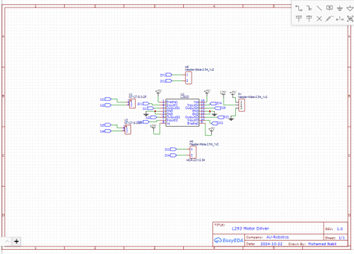
\includegraphics{media/circ1.png}
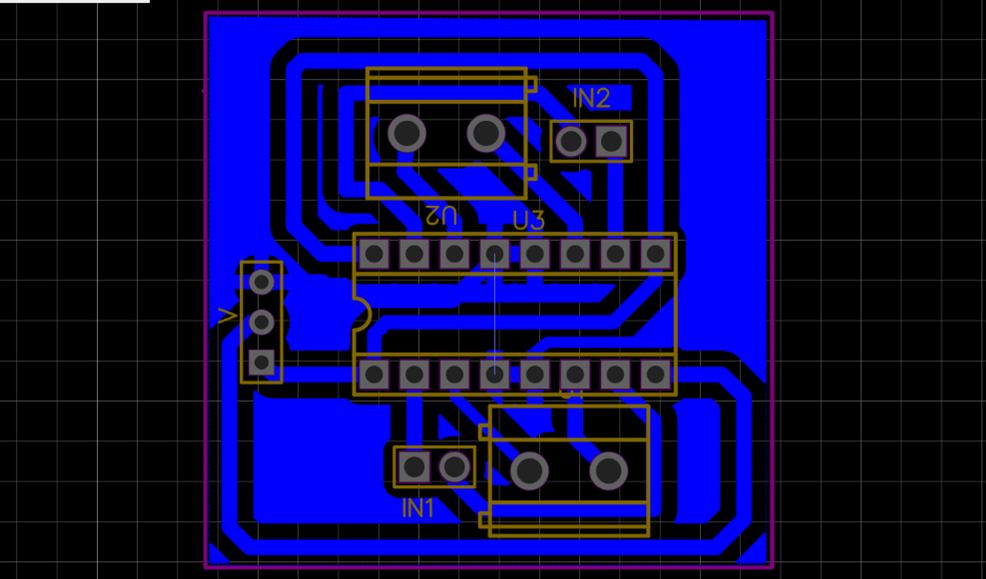
\includegraphics[trim=60 0 60 0, clip]{media/circ2.png}
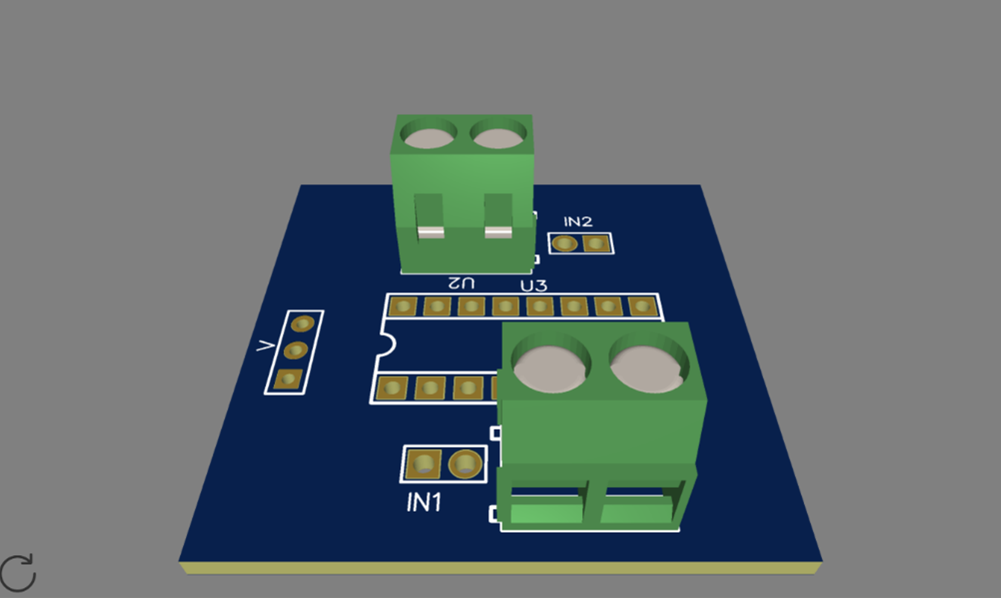
\includegraphics{media/circ3.png}

\end{document}